\section{隐通道构建}
\label{chap:zigzag:model}

本节对构建方法进行详细介绍,包括设计架构、调制流程及解调流程三个部分。设计架构部分,主要介绍该时间隐通道的主要流程,包含的处理环节及数据对象。调制流程部分,主要介绍调制过程中的流程、计算方法及数据处理流程。解调流程部分,主要介绍解调过程中,如何根据丢包序号还原隐蔽消息,包括数据转换及数据检验等部分。

\subsection{设计架构}
\label{chap:zigzag:model:system}

\insertFigure{
	\begin{figure}[htbp]
		\centering
        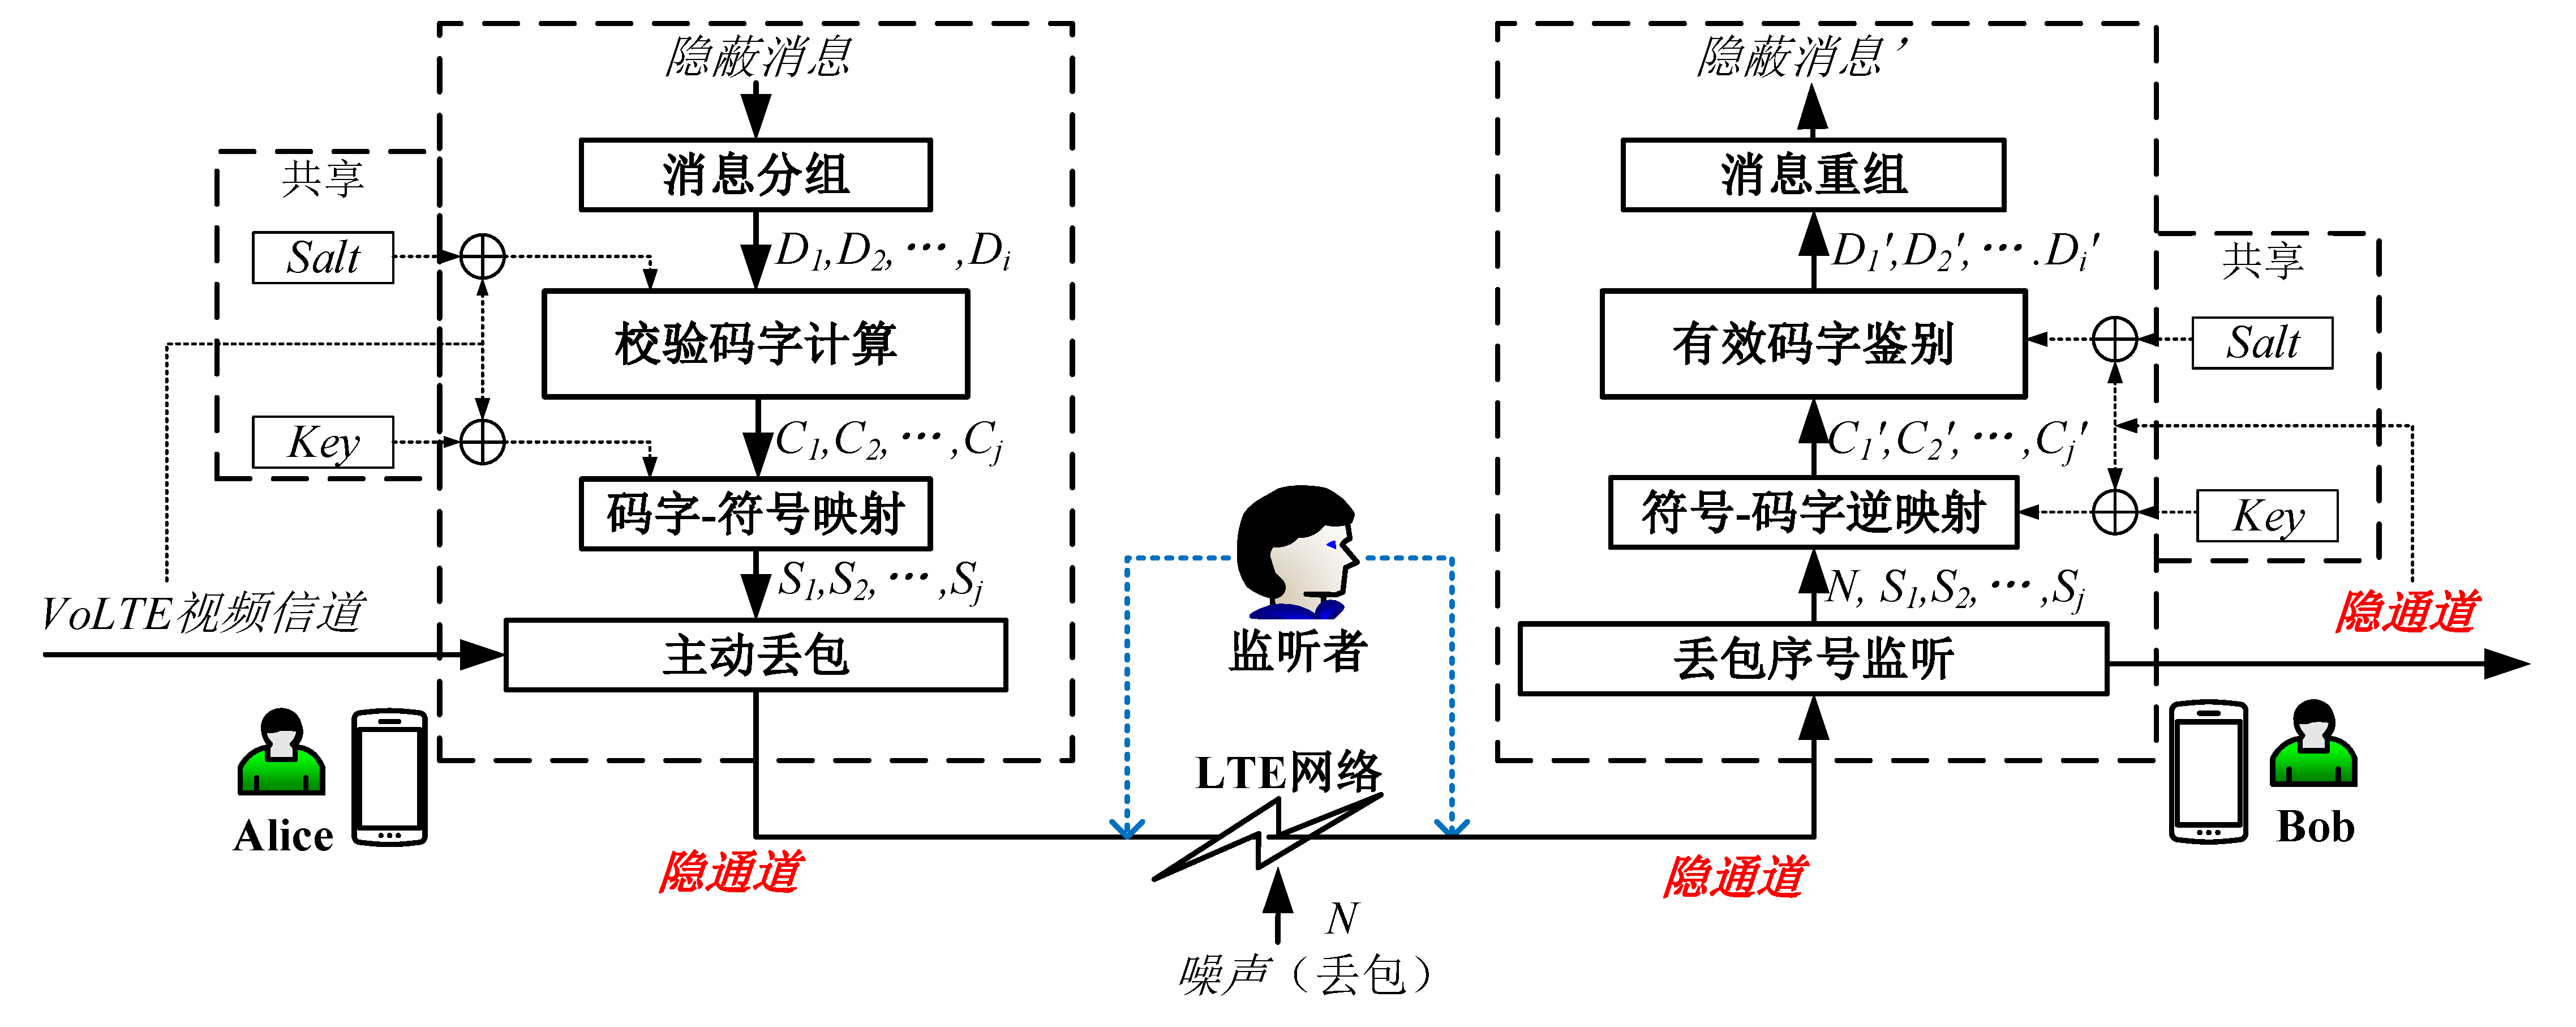
\includegraphics[width=0.98\textwidth]{chapters/chapter4/figures/system-model.pdf}
        \caption{基于Zigzag映射矩阵的时间隐通道系统模型图}
        \label{fig:4:system-model}
	\end{figure}
}

如图\ \nref{fig:4:system-model},对于用户Alice和Bob,希望通过该时间隐通道传输隐蔽消息,而监听者对两人的所有通信进行了监听,只允许被监听的VoLTE通话。在进行传输前,接收方与发送方预先约定共享的$Key$及$Salt$,类似消息加密的私有秘钥,分别用于映射矩阵初始化及CRC校验加盐。调制过程的消息分组阶段,完成对隐蔽消息的分组,生成定长的消息块$D_{i}$。校验码字计算阶段基于CRC算法,结合共享$Salt$及宿主信道的随机信息,计算码字校验值,生成所有码字$C_{j}$。码字-符号映射阶段,利用共享$Key$及随机信息初始化映射矩阵,并将码字$C_{j}$映射到相对序号$S_{j}$。主动丢包阶段,监控当前的数据包传输状态,并将目标数据包直接丢弃。

VoLTE数据包经LTE网络传输后,时间隐通道与网络噪声叠加。接收方通过监听RTP数据包序号,记录丢失数据包的序号。按照调制过程的逆序,解调过程识别符号$S_{j}^{'}$,然后参照逆映射矩阵将符号$S_{j}^{'}$转换为码字$C_{j}^{'}$,逆映射时映射矩阵的初始化参数与调制阶段保持一致。有效码字鉴别阶段根据CRC校验码字,筛选出符合校验规则的数据块$D_{i}^{'}$。最终消息重组阶段组合所有的消息块,得到隐蔽消息。

\subsection{调制流程}
\label{chap:zigzag:model:modulation}

\insertFigure{
	\begin{figure}[htb]
		\centering
        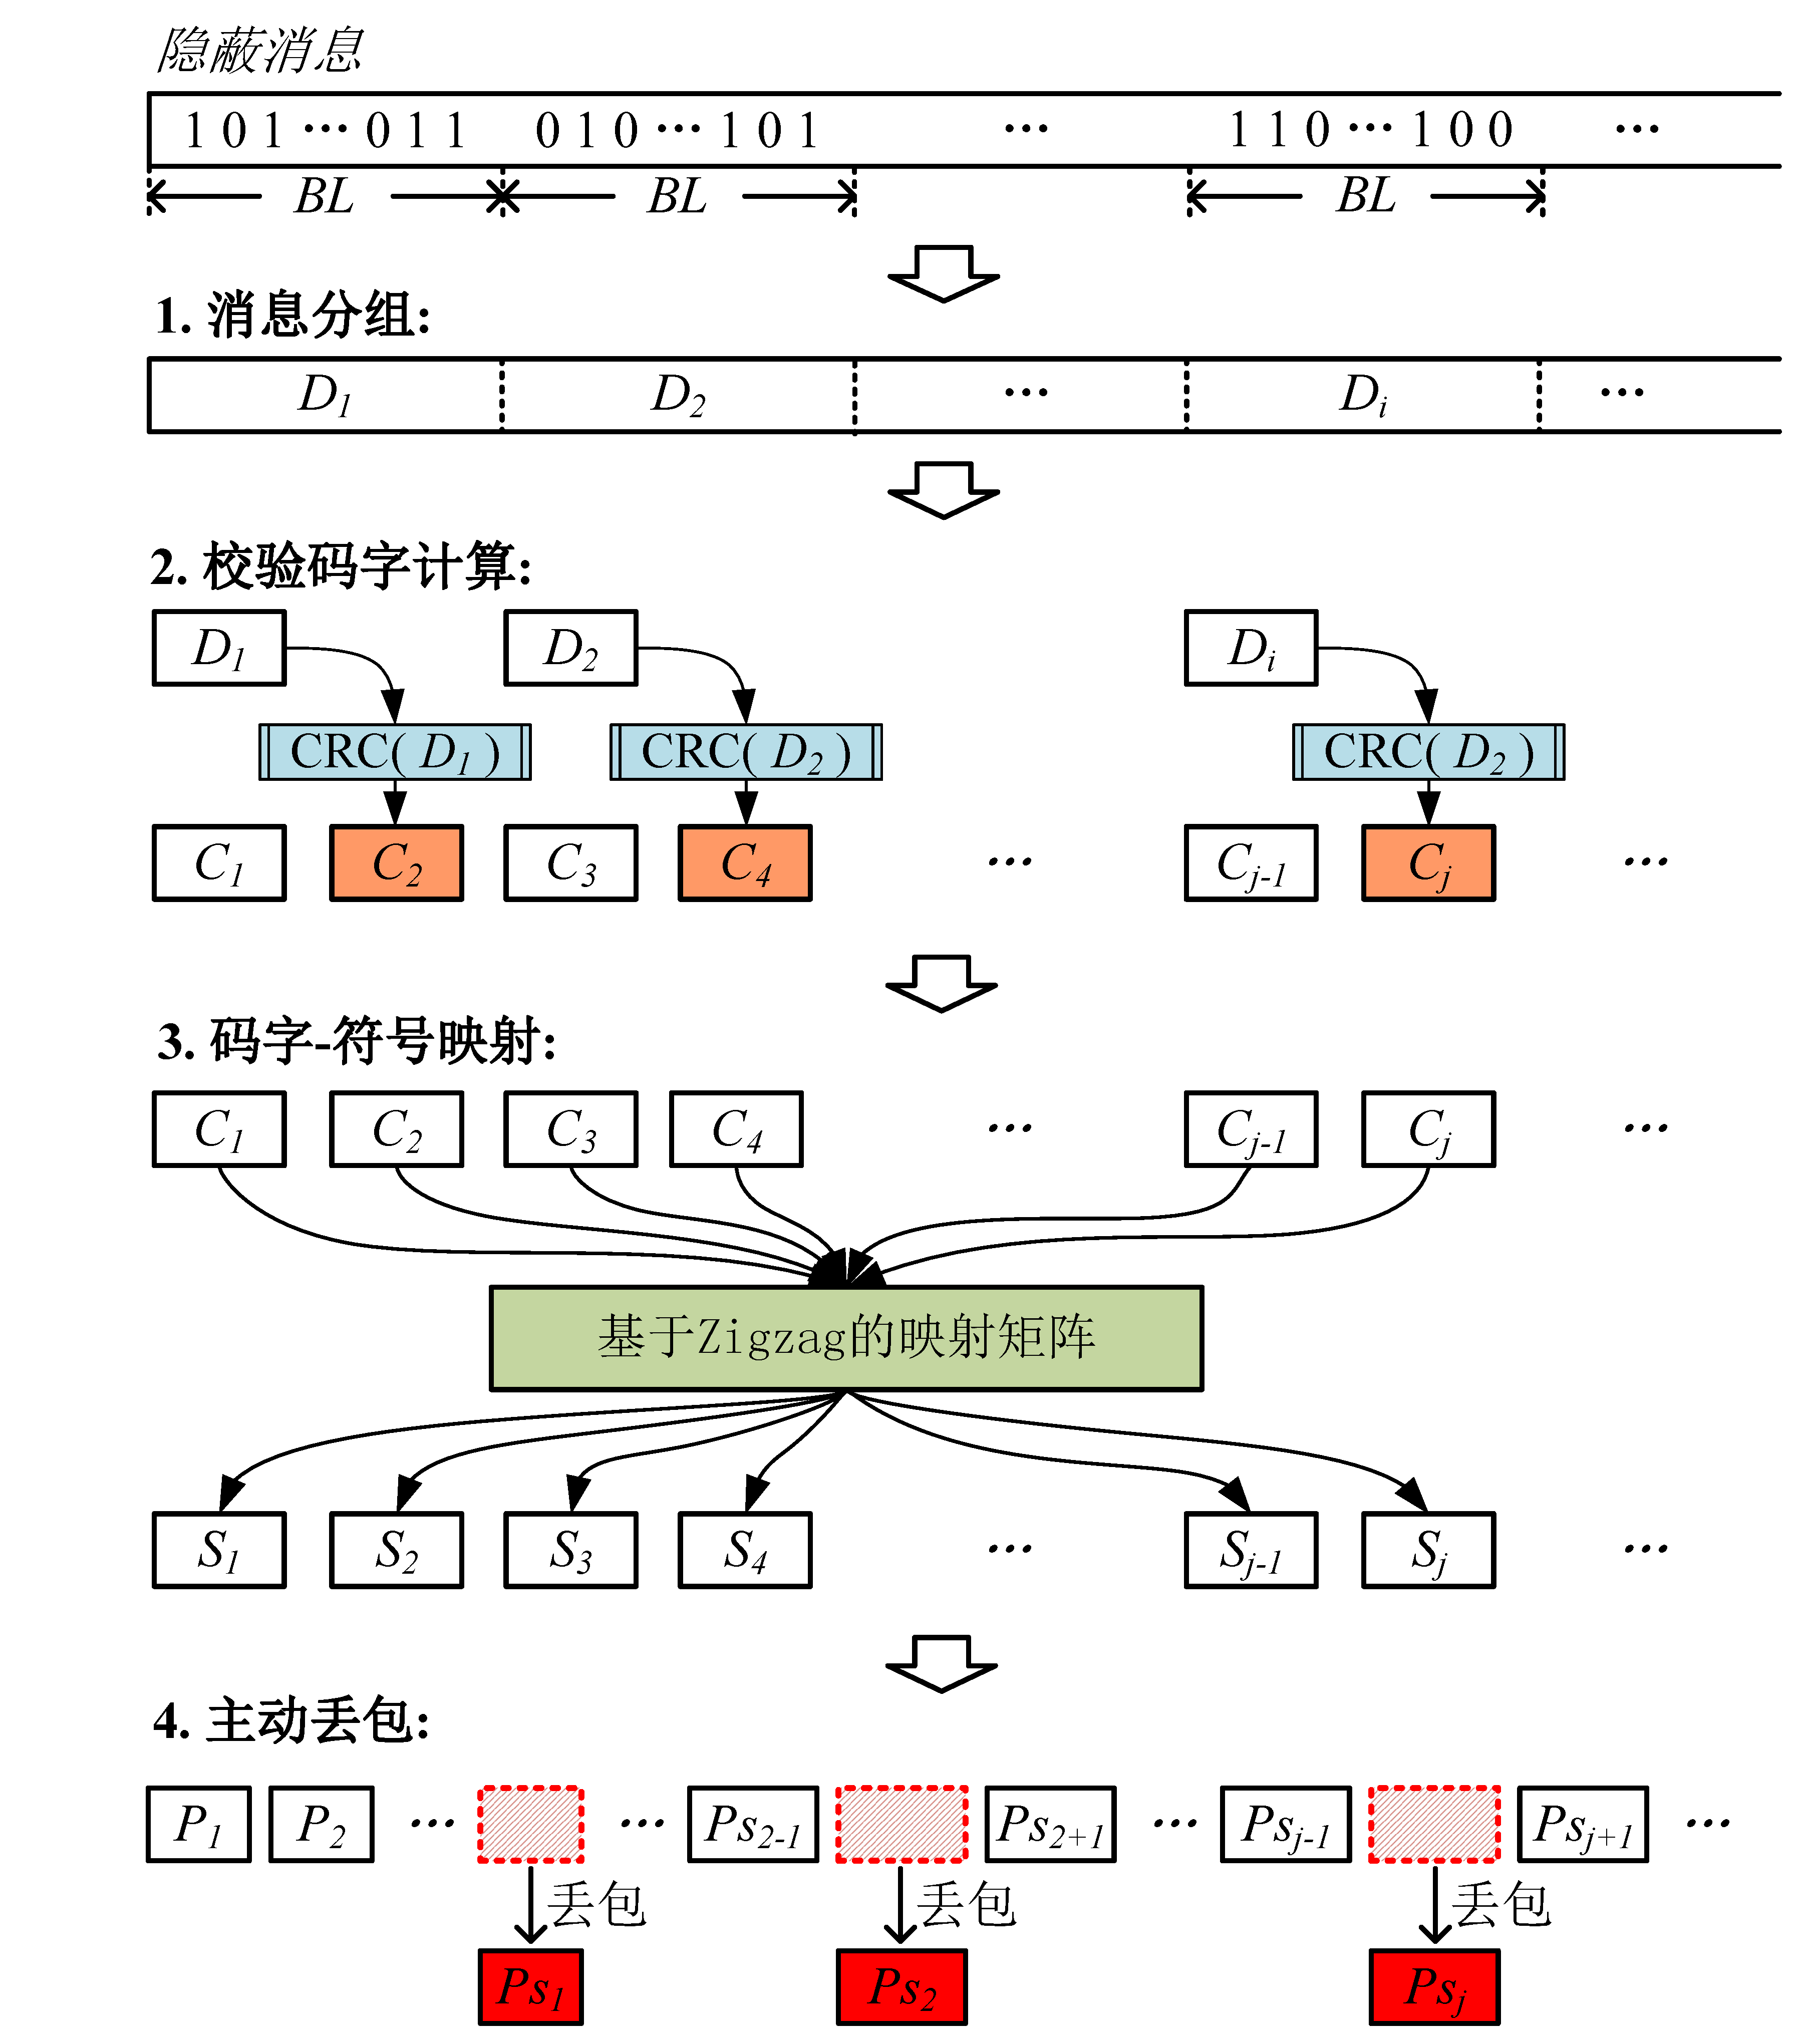
\includegraphics[width=0.8\textwidth]{chapters/chapter4/figures/modulation-flow.pdf}
        \caption{基于Zigzag映射矩阵的时间隐通道调制流程}
        \label{fig:4:modulation-flow}
	\end{figure}
}

如图\ \nref{fig:4:modulation-flow},调制过程中的处理步骤分为四个阶段,与系统模型中的各阶段对应。待发送的隐蔽消息为输入变量,最终结果是具有序号$S_{j}$的数据包被丢弃。

\subsubsection{隐蔽消息分组}
\label{chap:zigzag:model:modulation:segment}
隐蔽消息按照参数$BL$,切分为定长的消息块$D_{i}$,每个消息块单独调制。本方法中,码字未添加额外的校验信息,因此$L_{Codeword}=BL$。相对丢包位置与码字长度匹配,则传输每个码字需要的数据包数量为$2^{L_{Codeword}}$。
\insertEquation{
    \begin{equation}
    \label{equ:4:throughput}
    \begin{split}
        Throughput\ &=\ \frac{L_{Codeword}}{2^{L_{Codeword}\ +\ 1}}\ \times\ 100 \quad (bps)\ \\
        &=\ \frac{BL}{2^{BL\ +\ 1}}\ \times\ 100 \quad (bps)
    \end{split}
    \end{equation}
}

当确定了传输参数$L_{Codeword}$,则该时间隐通道的传输性能由公式(\nref{equ:4:throughput})计算,VoLTE视频数据包传输速率按照平均值$100\ (pkts/s)$。在有限的通话时间中,数据包总量是有限的,时间隐通道必须提高传输效率。该方法不需要同步时钟,提高了资源利用率。

\subsubsection{基于CRC的码字校验}
\label{chap:zigzag:model:modulation:crc}

基于CRC的码字校验,结合用户共享的$Salt$,以及由RTP传输流中导出的随机字段,生成唯一的校验码字。本方法中,选择RTP包头中的$SSRC$作为随机字段。$SSRC$与$Salt$异或后,与消息块$D_{i}$进行拼接,共同作为CRC函数的源数据。计算过程的描述如算法\ \nref{alg:4:codeword-generation},输入参数包括隐蔽消息及参数,最终返回生成的码字序列$C$。

\insertContents{
    \begin{algorithm}[htbp]
        \renewcommand{\algorithmcfname}{算法}
        \caption{码字生成}
        \label{alg:4:codeword-generation}
        \LinesNumbered
        \KwIn{$Covert\ Message,\ SSRC,\ Salt,\ L_{Codeword}$}
        \KwOut{$C\ \leftarrow\ \{\}$}
        $D\ \leftarrow\ \{\},\ offset\ \leftarrow\ 0$ \\
        \For {$offset\ <\ length\ (Covert\ Message)$} {
            $D_{i}\ \leftarrow\ Covert\ Message\ [offset\ :\ L_{Codeword}]$ \\
            append $\ D_{i}\ $ to $\ D$ \\
            $offset\ \leftarrow\ offset\ +\ L_{Codeword}$
        }
        $salt\ \leftarrow\ Salt\ \oplus\ SSRC$ \\
        \For {$D_i\ $ in $\ D$} {
            $C_{j}\ \leftarrow\ $CRC16\ ($salt\ //\ D_{i}\ //\ salt$) \\
            append $\ D_{i}\ $ to $\ C$ \\
            append $\ C_{j}\ $ to $\ C$
        }
        \Return $C$
    \end{algorithm}
}

\subsubsection{基于Zigzag矩阵的映射矩阵}
\label{chap:zigzag:model:modulation:mapping}

映射矩阵实现了码字$C_{j}$到符号$S_{j}$的转换,矩阵中元素数量由$L_{Codeword}$决定。矩阵的行数与列数如公式(\nref{equ:4:matrix-length})得出,映射矩阵$\textit{\textbf{M}}$为方阵,且满足$M_{cols}\times M_{rows}\ge 2^{L_{Codeword}}$。映射矩阵的映射关系,是本方法保密性的重要环节。图\ \nref{fig:4:zigzag-matrix}中$\textit{\textbf{M}}_{1,\ 1}$设定为1,而实际应用中,$\textit{\textbf{M}}_{1,\ 1}$由用户设定的$Key$及RTP中的随机字段决定,计算方法如公式(\nref{equ:4:matrix-begin})。映射矩阵排布完毕后,对每个元素$\textit{\textbf{M}}_{i,\ j}$取模,确保不超过上限$2^{L_{Codeword}}$。
\insertEquation{
    \begin{equation}
    \label{equ:4:matrix-length}
		M_{cols}\ =\ M_{rows}\ =\ 2^{\left \lceil \frac{L_{Codeword}}{2} \right \rceil}
    \end{equation}
    \begin{equation}
    \label{equ:4:mapping}
        S_{j}\ =\ \textit{\textbf{M}}_{C_{j,\ \lbrack L_{Codeword}/2,\ L_{Codeword})},\ C_{j,\ \lbrack 0,\ L_{Codeword}/2)}}
    \end{equation}
    \begin{equation}
    \label{equ:4:matrix-begin}
    \textit{\textbf{M}}_{1,\ 1}\ =\ (Key\ \oplus\ SSRC)\ \%\ 2^{L_{Codeword}}\ +\ 1
    \end{equation}
}

码字转换为符号的过程,由映射矩阵实现。对于码字$C_{j}$,其长度为$L_{Codeword}$\ bits,按照$L_{Codeword}/2$\ bits进行划分,得到前半部分$C_{j,\ [0,\ L_{Codeword}/2)}$,以及后半部分$C_{j,\ [L_{Codeword}/2,\ L_{Codeword})}$。参照图\ \nref{fig:4:zigzag-matrix}及映射矩阵初始化结果,按照公式(\nref{equ:4:mapping})完成转换。

\subsection{解调流程}
\label{chap:zigzag:model:demodulation}

\insertFigure{
	\begin{figure}[htb]
		\centering
        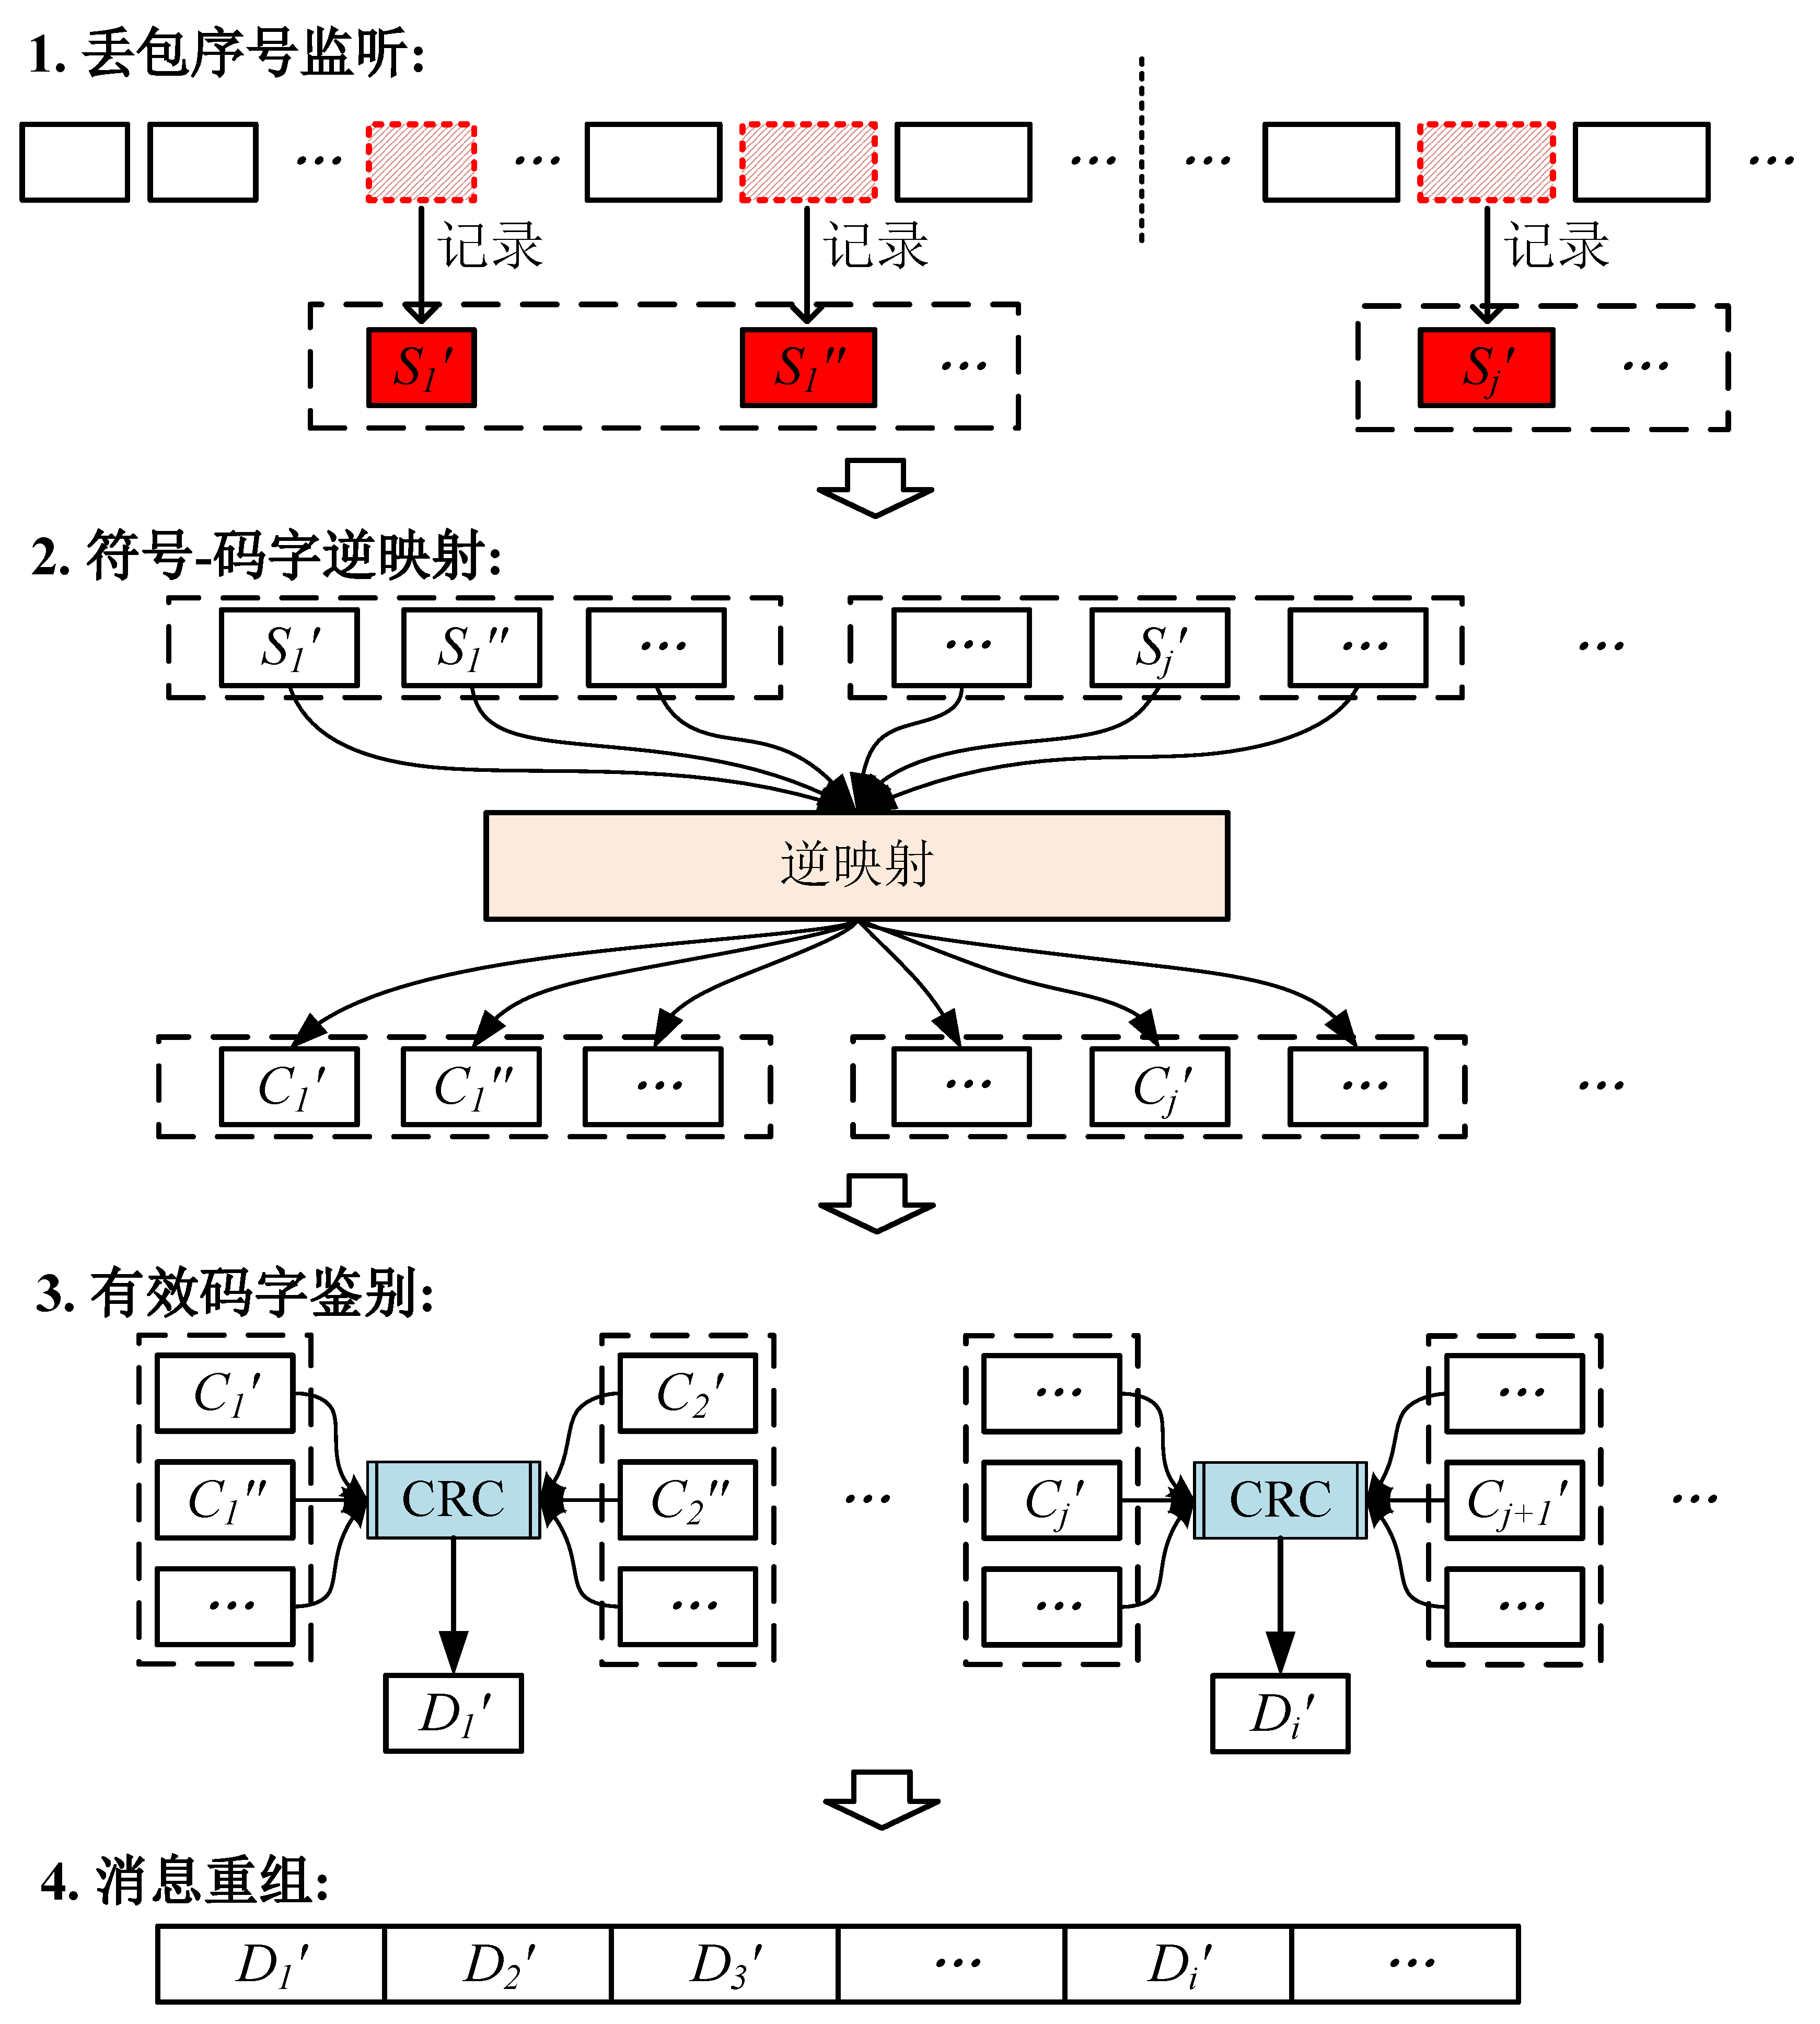
\includegraphics[width=0.8\textwidth]{chapters/chapter4/figures/demodulation-flow.pdf}
        \caption{基于Zigzag映射矩阵的时间隐通道解调流程}
        \label{fig:4:demodulation-flow}
	\end{figure}
}

如图\ \nref{fig:4:demodulation-flow},解调流程分为四个部分,包括丢包序号监听、符号-码字逆映射、有效码字鉴别,以及消息重组。由于网络噪声不可避免,解调过程中每组候选项不唯一,在验证结束前均为可行解。
\insertEquation{
    \begin{equation}
    \label{equ:4:group-id}
		j\ =\ \left \lfloor\frac{number\ -\ 1}{2^{L_{Codeword}}}\right \rfloor\ +\ 1
    \end{equation}
    \begin{equation}
    \label{equ:4:symbol}
        S_{j}\ =\ (number\ -\ 1)\ \%\ (2^{L_{Codeword}})\ +\ 1
    \end{equation}
}

根据映射矩阵的规模,每个矩阵对应的数据包数量为$2^{L_{Codeword}}$,则丢包序号$number$与$j$及$S_{j}$的对应关系如公式(\nref{equ:4:group-id})及公式(\nref{equ:4:symbol})。

\subsubsection{基于Zigzag矩阵的逆映射}
\label{chap:zigzag:model:demodulation:reverse-mapping}

映射矩阵将码字映射为符号,逆映射过程将符号还原为码字。对于接收方来说,通过映射矩阵进行逆映射效率较低,需要生成映射矩阵的逆映射关系。按照与调制过程相同的方式,构建映射矩阵的过程中,创建逆映射关系$S_{j}\ \rightarrow\ C_{j}$,通过索引快速完成逆映射。

\subsubsection{有效码字鉴别}
\label{chap:zigzag:model:demodulation:identification}

\insertContents{
    \begin{algorithm}[htbp]
        \renewcommand{\algorithmcfname}{算法}
        \caption{有效码字鉴别}
        \label{alg:4:codeword-identification}
        \LinesNumbered
        \KwIn{$\{\{C_{1}',\ \cdots\},\ \{C_{2}',\ \cdots\},\ \cdots\},\ Salt,\ SSRC$}
        \KwOut{$D'\ \leftarrow\ \{\}$}
        $salt\ \leftarrow\ Salt\ \oplus\ SSRC$ \\
        \For {$\{C_{j}',\ \cdots\},\ \{C_{j\ +\ 1}',\ \cdots\}\ $ in $\ C$} {
            \For {$C_{j}'\ $ in $\ \{C_{j}',\ \cdots\}$} {
                $checksum\ \leftarrow\ $CRC16\ ($salt\ //\ C_{j}'\ //\ salt$) \\
                \If {$checksum\ $ in $\ \{C_{j\ +\ 1}',\ \cdots\}$} {
                    append $\ C_{j}'\ $ to $\ D'$ \\
                    \textbf{break}
                }
            }
        }
        \Return $D'$
    \end{algorithm}
}

调制过程中,码字规模$j$是数据块规模$i$的2倍,即$j\ =\ 2\ \times\ i$。因此,解调过程中,码字划分为两部分,分别为奇数组的数据码字及偶数组的校验码字。如图\ \nref{fig:4:demodulation-flow},鉴别码字的过程中,通过重新计算校验值,判断校验值是否在校验码字中出现,从而判断数据码字的有效性。

码字鉴别过程的描述如算法\ \nref{alg:4:codeword-identification},首先计算盐值$salt$,由用户共享的$Salt$及随机字段$SSRC$组成。接下来,重新计算$C_{j}'$对应的校验码字,如结果在$\{C_{j\ +\ 1}',\ \cdots\}$中出现,则意味着$C_{j}'$符合校验规则。符合校验规则的$C_{j}'$加入到结果$D'$中,即为解调得到的有效数据块。最终,组合所有的数据块$D_{i}'$,还原隐蔽消息,解调过程结束。